\documentclass{article}
\PassOptionsToPackage{numbers,sort&compress}{natbib}
\usepackage[preprint]{neurips_2026}
\usepackage[T1]{fontenc}
\usepackage[utf8]{inputenc}
\usepackage{amsmath,amssymb,booktabs,graphicx}
\usepackage{hyperref}
\hypersetup{hidelinks}
% Presentation only; source CSV statistics are unchanged.
\newcommand{\EntryContrast}{-0.1986}
\newcommand{\EntryLow}{-0.2494}
\newcommand{\EntryHigh}{-0.1485}
\newcommand{\EntryCrossLow}{-0.4255}
\newcommand{\EntryCrossHigh}{+0.0179}
\newcommand{\RecoveryContrast}{+0.0069}
\newcommand{\RecoveryLow}{-0.0052}
\newcommand{\RecoveryHigh}{+0.0192}
\newcommand{\RecoveryCrossLow}{-0.0589}
\newcommand{\RecoveryCrossHigh}{+0.0673}
\newcommand{\PanelReadout}{%
\begin{tabular}{lrrr}
\toprule
Phase & Panel 1 & Panel 2 & Panel 3 \\
\midrule
Entry & -0.3101 & -0.2547 & -0.0309 \\
Recovery64 & -0.0110 & -0.0107 & +0.0425 \\
\bottomrule
\end{tabular}}
\newcommand{\ComponentReadout}{%
\begin{tabular}{llrrr}
\toprule
Model & Phase & Total & Current & Archive \\
\midrule
GRU & Entry & -0.2071 & -0.1302 & -0.0769 \\
GRU & Recovery64 & -0.0326 & +0.0504 & -0.0830 \\
TCN & Entry & -0.0085 & +0.0611 & -0.0697 \\
TCN & Recovery64 & -0.0396 & +0.0210 & -0.0606 \\
\bottomrule
\end{tabular}}
\newcommand{\VariabilityCount}{4}
\newcommand{\VariabilityComparisons}{6}
\newcommand{\AbsoluteReadout}{%
\begin{tabular}{llrrr}
\toprule
Model & Interval & Score & Coverage & Width \\
\midrule
GRU & Native & 4.986 & 94.42\% & 4.544 \\
GRU & W32 & 5.245 & 91.48\% & 4.439 \\
GRU & W128 & 5.299 & 95.09\% & 4.902 \\
TCN & Native & 4.938 & 94.26\% & 4.470 \\
TCN & W32 & 5.229 & 91.66\% & 4.452 \\
TCN & W128 & 5.283 & 95.16\% & 4.887 \\
\bottomrule
\end{tabular}}

% Display only. Complete rank and FX outcomes remain in saved CSVs.

\newcommand{\RankReadout}{%
\begin{tabular}{lrrr}
\toprule
Phase & Original rank & Randomized rank & Change \\
\midrule
Entry & -0.1986 & -0.1946 & +0.0040 \\
Recovery64 & +0.0069 & +0.0043 & -0.0027 \\
\bottomrule
\end{tabular}}

\newcommand{\FXMainReadout}{%
\begin{tabular}{lrrrr}
\toprule
& \multicolumn{2}{c}{Native} & \multicolumn{2}{c}{Rolling128} \\
Model & Coverage & IS & Coverage & IS \\
\midrule
GRU & 90.05\% & 3.178 & 90.70\% & 3.219 \\
TCN & 91.01\% & 3.166 & 90.68\% & 3.204 \\
GARCH & 92.78\% & 3.240 & 90.45\% & 3.192 \\
\bottomrule
\end{tabular}}

\newcommand{\FXFullReadout}{%
\begin{tabular}{lrrrrrr}
\toprule
Model & Native & W32 & W128 & ACI128 & SF-OGD & SAOCP \\
\midrule
Constant & 3.740 & 3.226 & 3.244 & 3.222 & 3.232 & 3.298 \\
EWMA16 & 3.168 & 3.373 & 3.222 & 3.287 & 3.373 & 3.545 \\
EWMA64 & 3.195 & 3.277 & 3.218 & 3.267 & 3.288 & 3.395 \\
GARCH & 3.240 & 3.288 & 3.192 & 3.249 & 3.292 & 3.427 \\
GRU64 & 3.178 & 3.374 & 3.219 & 3.284 & 3.355 & 3.495 \\
TCN64 & 3.166 & 3.342 & 3.204 & 3.261 & 3.319 & 3.450 \\
\bottomrule
\end{tabular}}

\newcommand{\FXMechanismReadout}{%
\begin{tabular}{lrrr}
\toprule
Model & $J_{\rm FX}$ & $C_{b64}$ & $A_{a16}$ \\
\midrule
GRU & -0.0061 & +0.0145 & -0.0206 \\
TCN & +0.0171 & +0.0175 & -0.0004 \\
GRU$-$TCN & -0.0232 & -0.0030 & -0.0202 \\
\bottomrule
\end{tabular}}

\title{Separating Neural Scale Response and Score Memory\\in Online Interval Calibration}
\author{Chengxuan YUAN (50025581)\\DSAA 2012, HKUST(GZ)\\Working draft for student review, 18 October 2026}
\begin{document}
\maketitle
\begin{abstract}
Normalized-score calibration combines a neural forecaster's current scale with
historical forecast errors divided by their originally issued scales. We study
these two pathways separately in paired volatility-pulse simulations, keeping
trained weights fixed and using the same observations across configurations.
An initial five-seed GRU/TCN comparison is sensitive to training randomness.
We replicate with three new training datasets and five paired seeds per dataset,
retaining both current-scale and archived-score decomposition orders.
The entry architecture contrast keeps its direction across new datasets, but
training-randomness sensitivity still includes zero; the recovery contrast
does not replicate reliably. In the reference Gaussian entry comparison,
TCN has greater current-channel seed variability than GRU, while archive
variability can dominate within a dataset.
A post-hoc common-rank-level check retains the negative mean Gaussian entry contrast while
revealing sensitivity in smaller effects. A separate public-FX extension
compares absolute interval quality and descriptive pathway differences.
These findings do not establish a general architecture ranking or a
coverage guarantee; all fitted models and failed replication outcomes remain.
\end{abstract}

\section{Research question and contribution scope}
Financial uncertainty intervals should expand when risk rises and contract
when a temporary disturbance ends. A learned scale model and an online
calibrator can each retain information about that disturbance. Their
combination may behave differently from either component alone.
We ask: \emph{where does variability across fitted neural models enter
normalized-score calibration at shock entry and recovery?}

This controlled deep-learning study learns scales from raw past returns;
a zero center isolates uncertainty adaptation. It examines a computational
pathway without establishing trading gains or deployable conditional coverage.

Underspecification already explains why strong in-domain validation need not
constrain deployment behavior \citep{damour}; HARNet studies initialization
stability in neural volatility prediction \citep{harnet}. Neural conformal
control \citep{ncc}, jointly adapting scores and thresholds \citep{adapt},
retrospective residual updates \citep{retro}, strongly adaptive experts
\citep{saocp}, and scorecasting with feedback \citep{pid} are established.
We do not claim these ideas as new.
AdaptNC updates score parameters with replay; RetroAdj recomputes
leave-one-out residuals. Our experiment fixes neural weights and separately
varies current and archive contexts.

The intended increment is an explicit separation of \emph{current neural
scale} and \emph{historically issued score denominators}, with paired
observations, two decomposition orders, and independent training-data
repeats. The initial crossed analysis was exploratory; its specific
replication questions were fixed before new training and test generation.
Evidence that fails to replicate must narrow the conclusion.

\clearpage
\section{Crossed pathways and evaluation}
For a fixed trained model, let $s_t^a>0$ be the scale predicted from the last
$a\in\{16,64\}$ observations, excluding $y_t$. Define
\begin{equation}
 q_t^{b,W}=\operatorname{OrderStat}_{k}
 \left\{\frac{|y_i|}{s_i^b}:i=t-W,\ldots,t-1\right\},
 \quad h_t^{a,b,W}=s_t^a q_t^{b,W},
 \quad k=\lceil(W+1)(1-\alpha)\rceil.
\end{equation}
Here $b\in\{16,64\}$, $W\in\{32,128\}$ and $\alpha=.1$.
The deployed diagonal has $a=b$; the full eight-cell factorial changes the
current and archive contexts independently. Warmup uses the last 128 scores
of a separate validation path, with predictor-specific issued denominators.

For each cell and phase, $E(a,b,W)$ is its event-minus-matched-control
mean interval score. Write $D(a,b)=E(a,b,128)-E(a,b,32)$. The diagonal
context-by-window interaction is $J=D(64,64)-D(16,16)$, and
\begin{align}
 J&=\underbrace{D(64,64)-D(16,64)}_{C_{b64}}
   +\underbrace{D(16,64)-D(16,16)}_{A_{a16}},\\
  &=\underbrace{D(64,16)-D(16,16)}_{C_{b16}}
   +\underbrace{D(64,64)-D(64,16)}_{A_{a64}}.
\end{align}
These are exact computational differences, not unique causal mediation
fractions. Correlated component interval endpoints cannot be added.
$C$ and $A$ are channel-by-window interaction components, not channel main effects.

\paragraph{Training and tests.}
The GRU \citep{gru} has 2041 parameters; the causal dilated TCN
\citep{tcn} has 1897 and receptive field 64. Both use features $(y/3,\log(1+|y|))$, Gaussian scale loss, two
contexts, data and paired sampler prefixes. Each target resets state.
Adam and validation early stopping are fixed; total optimization steps may
differ between architectures. Context length is not effective learned memory.
Training uses 256 paths of length 1024; validation uses 64 paths and 8192 shared
sampled targets. Each of three new datasets trains five seed pairs.
The original five seed indices are reused: independence refers to new
training/validation and test data, not 15 independent initialization/sampling draws.

The initial frozen grid has 30 cases: Gaussian, unit-variance t5 and stochastic
volatility, five pulse durations and two amplitudes. The new replication
fixes Gaussian/t5, amplitude 3 and durations 32/128, with 128 independent
paired paths per family. Pulses begin at 384; recovery64 follows their exit.
Families have separate noise streams; durations share their family stream,
so both duration conditions have identical entry32 and are not independent
replications. Event labels and true scales enter generation and evaluation
only, never the model or quantile.

\paragraph{Scores and uncertainty.}
We report interval score $2h+(2/\alpha)(|y|-h)_+$ \citep{gneiting},
coverage, width, oracle coverage deficit and excess width.
The two reference contrasts are GRU $J$ minus TCN $J$ for Gaussian D128/A3,
at entry and recovery64. The 4000-draw paired-path bootstrap averages all 15
fixed fitted pairs before resampling; 97.5\% marginal intervals provide a
two-phase Bonferroni approximation. Crossed dataset/seed/path resampling is
sensitivity only: shared seed draws stay shared across datasets, with only
three datasets and five seeds. Secondary intervals are descriptive.
Finite quantile ranks also differ: ideal continuous exchangeable-score
coverage is 30/33 for W32 and 117/129 for W128. The contrast therefore includes
rank discretization as well as history length; this benchmark is not a
coverage guarantee for our dependent scores.

\clearpage
\section{Results and interpretation}
\paragraph{Initial study motivated replication.}
In the initial five-seed Gaussian D128/A3 study, GRU-minus-TCN $J$ is
$-0.05287$ at entry and $+0.03276$ at recovery64.
Fixed-fit 97.5\% intervals exclude zero, but crossed seed/path intervals
include zero. The entry seed range is $[-0.42866,+0.47620]$;
omitting one seed can reverse the mean.

\paragraph{Independent training-data replication.}
With 15 new paired fits, the reference contrasts are
$\EntryContrast$ at entry, fixed-fit 97.5\% interval
$[\EntryLow,\EntryHigh]$, and $\RecoveryContrast$ at recovery64,
interval $[\RecoveryLow,\RecoveryHigh]$.
Crossed sensitivity ranges are
$[\EntryCrossLow,\EntryCrossHigh]$ and
$[\RecoveryCrossLow,\RecoveryCrossHigh]$.
All initialization outcomes remain in the analysis; these are interactions,
not absolute interval-score rankings.
Entry has the same negative mean direction in all three datasets, but the
crossed interval includes zero. Recovery changes direction across datasets;
omitting panel 3 reverses its mean. The earlier positive recovery contrast
therefore did not replicate reliably.

\begin{center}
\PanelReadout
\end{center}
\noindent Entries average five paired seeds per new training-data panel.
Shared seeds and test paths preclude six independent significance tests.

\begin{figure}[h]
\centering
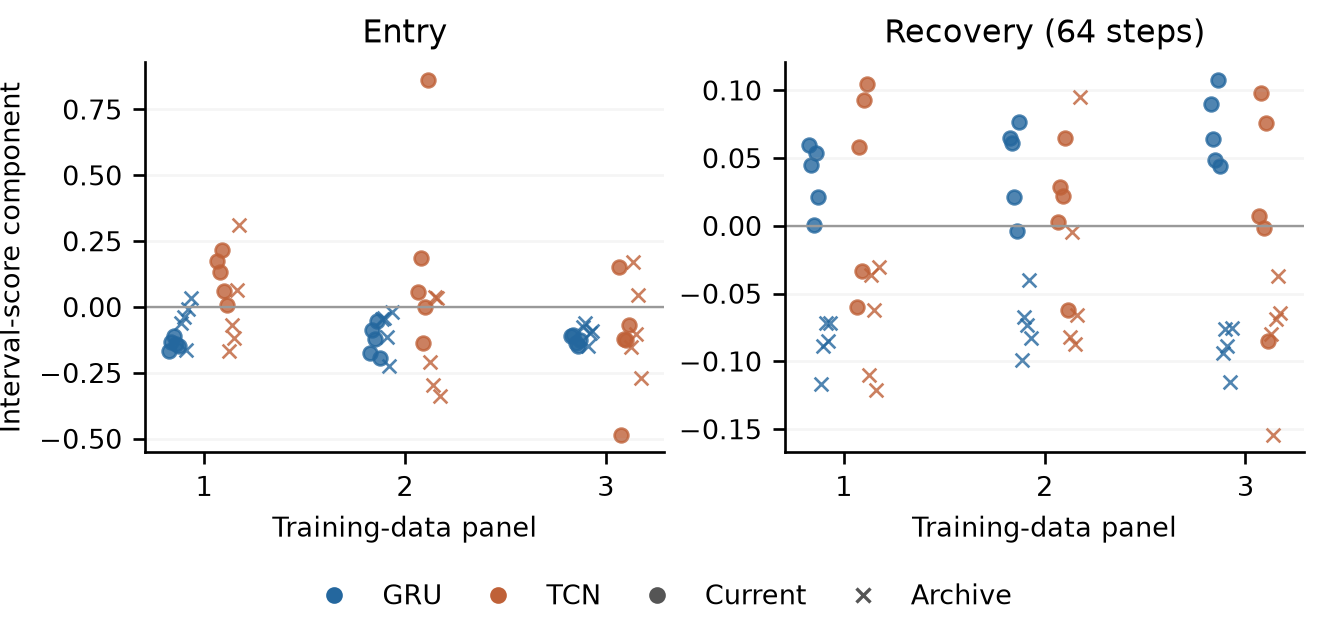
\includegraphics[width=\linewidth]{stage3_components.png}
\caption{All five seeds per architecture and new dataset, Gaussian D128/A3.
Current circles denote $C_{b64}$ and archive crosses $A_{a16}$.
Point spread describes training variability, not causal variance attribution.}
\end{figure}

\noindent TCN entry current seed standard deviation exceeds GRU's in all six
panel-by-route comparisons, but exceeds its own archive spread in only
$\VariabilityCount/\VariabilityComparisons$. Panel 1 has larger archive
spread in both routes. These correlated comparisons are descriptive;
Appendix A retains the component means and absolute interval costs.

\paragraph{Interpretation requires the score as well as the response.}
A small total can conceal opposing components. At recovery, GRU's
$C_{b64}=+0.0504$ and $A_{a16}=-0.0830$ partly cancel; TCN's are
$+0.0210$ and $-0.0606$. Moreover, the mixed derivative of expected Gaussian
interval score for $h=sq$ changes sign (Appendix A). Thus signed $J$ combines
scale response, archive quantiles and score curvature; it cannot label
memory as beneficial or harmful. Neither the algebraic decomposition nor
the finite input-dependency bound is presented as a novel theorem.

\clearpage
\section{Sensitivity, financial extension, and boundaries}
\paragraph{Finite-rank sensitivity on the same saved paths.}
We freeze a post-hoc check using all 30 Stage3 models and the already-viewed
Gaussian/t5 D128/A3 paths. A randomized rule uses ranks 29/30 with
probabilities .30/.70 at W32, and 116/117 with .90/.10 at W128. Both have
ideal exchangeable-score rank level .90. We integrate each candidate
interval's \emph{metric}, not its width before scoring. This lowers both
original ideal rank levels. Within either rule, comparing W32 with W128
still changes score count and history span. This is rule sensitivity,
not causal removal of a discretization effect.

\begin{center}
\RankReadout
\end{center}
\noindent Entries are GRU-minus-TCN $J$ for Gaussian; the change uses paired
rules on common bootstrap draws. Fixed-fit 97.5\% change intervals are
$[-0.0124,+0.0210]$ at entry and $[-0.0103,+0.0048]$ at recovery.
Crossed sensitivity intervals still contain zero; recovery panel directions
remain mixed. TCN's own near-zero entry mean changes sign. For t5 recovery,
the GRU-minus-TCN contrast changes by $+0.00936$ with fixed-fit 95\% interval
$[+0.00230,+0.01661]$, but crossed $[-0.00322,+0.02139]$.
Rank choice therefore matters for some smaller quantities. This check
cannot repair the failed independent recovery replication.

\paragraph{Public FX: absolute quality and a descriptive contrast.}
We use the same frozen ECB \citep{ecb} USD/JPY/GBP/CHF-per-EUR archive through
9 October 2026. Training and per-asset standardization use data through
2018; checkpoint selection and calibrator-scale preparation use 2019.
Each currency replays its own 2020 history before scoring the already-viewed
2021--2026 period. Ten new pooled GRU/TCN fits retain all five paired seeds.
Training-only constant, EWMA16/64 and GARCH scales provide classical controls.
Native, rolling32/128, ACI \citep{aci}, author SF-OGD and SAOCP comparisons are retained
(Appendix B); no test-based winner or event subset is selected.

\begin{center}
\FXMainReadout
\end{center}
\noindent Context64 neural results average seeds, then currencies; IS is
in training-standard-deviation units. Columns were chosen before the new
run; Appendix B includes all six calibrators. Both neural models have lower native mean IS than GARCH. Under every
online calibrator, their pooled mean IS is higher than GARCH's; uncertainty
varies by comparison. This reversal motivates evaluating predictor--calibrator
combinations rather than declaring a general neural advantage.

For FX, $D_{\rm FX}(a,b)$ is the observed mean score difference W128-minus-W32,
and $J_{\rm FX}=D_{\rm FX}(64,64)-D_{\rm FX}(16,16)$, with both decomposition
orders retained. There is \emph{no matched control or known shock/recovery}
on this history. Joint date-block intervals preserve shared currency dates
and are conditional on the saved fits; four correlated currencies and five
seeds are not independent market histories.

\paragraph{Scope.}
Evidence is specific to small zero-center neural scale models, a fixed
training procedure, the simulated generator and one viewed FX archive.
The study supports a reproducible separation of computational pathways and
identifies where apparent contrasts fail to generalize across fits or
settings. It establishes neither deployable coverage nor trading gains.
Training-randomness uncertainty and the recovery failure remain central,
regardless of additional sensitivity checks.

\clearpage
\begingroup
\raggedright
\begin{thebibliography}{99}
\bibitem[D'Amour et~al.(2022)]{damour}
A. D'Amour et al. Underspecification Presents Challenges for Credibility in
Modern Machine Learning. \emph{JMLR}, 23(226):1--61, 2022.
\url{https://jmlr.org/papers/v23/20-1335.html}
\bibitem[Reisenhofer et~al.(2022)]{harnet}
R. Reisenhofer, X. Bayer, and N. Hautsch. HARNet: A Convolutional Neural
Network for Realized Volatility Forecasting. arXiv:2205.07719, 2022.
\bibitem[Li and Rodr\'iguez(2025)]{ncc}
R. Li and A. Rodr\'iguez. Neural Conformal Control for Time Series
Forecasting. \emph{AAAI}, 39(17):18439--18447, 2025.
\bibitem[Tumu et~al.(2026)]{adapt}
R. Tumu, A. Singh, and R. Mangharam. AdaptNC: Adaptive Nonconformity Scores
for Conformal Prediction under Distribution Shift. arXiv:2602.01629v2, 2026.
\bibitem[Jun and Ohn(2026)]{retro}
J. Jun and I. Ohn. Online conformal inference with retrospective adjustment
for faster adaptation to distribution shift.
\emph{Pattern Recognition}, 180:114406, 2026.
\bibitem[Bhatnagar et~al.(2023)]{saocp}
A. Bhatnagar, H. Wang, C. Xiong, and Y. Bai.
Improved Online Conformal Prediction via Strongly Adaptive Online Learning.
\emph{ICML}, PMLR 202:2337--2363, 2023.
\bibitem[Angelopoulos et~al.(2023)]{pid}
A. N. Angelopoulos, E. J. Cand\`es, and R. J. Tibshirani.
Conformal PID Control for Time Series Prediction. \emph{NeurIPS}, 2023.
\bibitem[Gneiting and Raftery(2007)]{gneiting}
T. Gneiting and A. E. Raftery. Strictly Proper Scoring Rules, Prediction,
and Estimation. \emph{JASA}, 102(477):359--378, 2007.
\url{https://doi.org/10.1198/016214506000001437}
\bibitem[Cho et~al.(2014)]{gru}
K. Cho et al. Learning Phrase Representations using RNN Encoder-Decoder
for Statistical Machine Translation. \emph{EMNLP}, 2014. arXiv:1406.1078.
\bibitem[Bai et~al.(2018)]{tcn}
S. Bai, J. Z. Kolter, and V. Koltun. An Empirical Evaluation of Generic
Convolutional and Recurrent Networks for Sequence Modeling.
arXiv:1803.01271, 2018.
\bibitem[Gibbs and Cand\`es(2021)]{aci}
I. Gibbs and E. J. Cand\`es. Adaptive Conformal Inference Under
Distribution Shift. arXiv:2106.00170, 2021.
\bibitem[European Central Bank(2026)]{ecb}
European Central Bank. Euro foreign exchange reference rates.
Frozen historical archive ending 9 October 2026.
\url{https://www.ecb.europa.eu/stats/eurofxref/eurofxref-hist.zip}
\end{thebibliography}
\endgroup


\section*{Reproducibility and draft status}
Frozen protocols, checkpoints, complete metrics and source/input hashes are
available at \url{https://github.com/Lebmar/DL-project/tree/codex/stage2-memory-study}.
Writers refuse silent overwriting. Stage3 statistics remain unchanged;
new sensitivity and FX displays are read from their separately saved outputs.
Main text ends on page 4; references and appendices are extra.
AI tools assisted implementation, checking and drafting with course permission.
This is a working report for the student's interpretation and revision;
it has not been submitted by the assistant.

\clearpage
\appendix
\section{Synthetic design and interpretation details}
\paragraph{Fixed training procedure.}
All synthetic models use GRU hidden size 24 or TCN 12 channels with kernels
$(4,3,3,3,3)$ and dilations $(1,2,4,8,16)$, clipped log-scale $[-3,3]$,
Adam learning rate .002, gradient norm clipping at 5, batch size 128 and
32 balanced-context batches per epoch. Validation chooses the absolute
minimum NLL; patience 8 uses tolerance $10^{-4}$ after at least 20 epochs,
with maximum 60. Shared sampler prefixes do not imply equal stopping times.
The three Stage3 training seeds are 314259/314359/314459, with separate
validation seeds and target-pair seeds; each panel reuses fit seeds
4101--4105. Protocols identify all generator and evaluation seeds.

\paragraph{Implementation checks.}
Stage3 verifies 480 diagonal cells and 960 crossed finite-memory controls.
If event/control observations agree from exit $e$, a fixed current context
$a$, archive context $b$ and window $W$ give identical half-widths from
$e+\max(a,b+W)$. This is an input-dependency check; persistent adaptive
controller states need not obey it. It does not assert market recovery
within 192 days. TCN64 full-sequence inference is checked against reset
windows before test access. Canonical pulse horizons preserve identical
entry prefixes across durations. Saved-output audits reproduce validation
losses, sampling digests, stopping decisions and response features.

\paragraph{Component means and absolute interval quality.}
The first table uses Gaussian D128/A3 and all 15 fits per architecture,
with route $C_{b64}+A_{a16}$; the second uses context64 recovery64 event
paths. Higher coverage can accompany wider intervals and a worse score.
\begin{center}
\ComponentReadout
\end{center}
\begin{center}
\AbsoluteReadout
\end{center}

\paragraph{Standard score geometry.}
For Gaussian $Y\sim N(0,\tau^2)$, expected interval score is
\[
 R(h;\tau)=2h+\frac{4}{\alpha}
 \{\tau\phi(h/\tau)-h\,\overline\Phi(h/\tau)\}.
\]
With $h=sq$ and $z=h/\tau$, the mixed derivative
$R_h+hR_{hh}=2-(4/\alpha)\{\overline\Phi(z)-z\phi(z)\}$ changes sign.
A fixed-archive scale-by-quantile contrast is its oriented rectangle
integral. These calculus facts explain why a signed interaction need not
rank memory quality. An earlier seed4101 Gaussian/t5 innovation-integration
check preserves its interaction directions but says nothing decisive
about initialization variability.

\paragraph{Validation probes and rank checks.}
All 30 models retain raw-input gradients and older-block permutations on
256 saved validation targets, plus 64 separate validation pulse paths.
Panel-specific scatterplots are exploratory: no equivalence test,
meta-regression or predictive model selection was performed.
For rank sensitivity, all 92,160 original per-path components and 1,920
crossed cell means reproduce Stage3 within $1.8\times10^{-15}$; 960
candidate-rank negative controls pass. Randomization is integrated after
each nonlinear metric, including positive-part oracle deficits. New common
bootstrap draws support paired rule changes, so original-rule bootstrap
endpoints differ slightly from the historical Stage3 table while point
estimates and raw outputs remain unchanged. The 97.5\% intervals adjust
for two phases separately within each rule/change series, not jointly
across rules. Secondary 95\% intervals are unadjusted; all rank analyses
remain post hoc.

\clearpage
\section{Financial extension and complete comparisons}
\paragraph{Data and chronology.}
Each currency's percentage log return $100\log(P_t/P_{t-1})$ is divided,
without demeaning, by its training standard deviation (ddof1). The archive
contains informational reference prices, not point-in-time vintages or
executable prices. Ten pooled neural fits use Appendix A's models and
optimizer, uniform currency sampling and seeds 4301--4305 on local CPU.
Both contexts select one common checkpoint by 2019 NLL. Classical scales
recurse continuously across boundaries; calibrators have separate states
for each currency and forecast stream.

ACI uses $\gamma=.02$ and window128 with clipped error rate. Author
SF-OGD/SAOCP use $\sqrt3\max_{2019}|y|/s$ as the fixed scale heuristic,
without clipping scores; 29 of 56 distinct streams exceed it during replay.
SAOCP lifetime is 8. Observed 2020 outcomes update
calibration but are excluded from reported metrics; 2021 begins without
resets. Strong controllers use all ten context64 fits. Native/rolling/ACI
retain both contexts, including all eight rolling crossed cells.

\paragraph{Complete context64 absolute-score table.}
\begin{center}
\FXFullReadout
\end{center}

\noindent Entries are means of per-date IS in per-currency training-standard-
deviation units, averaging neural seeds before equal currency weights.
All corresponding coverage, width, per-currency, annual and individual-fit
results remain in the saved tables; 2026 is partial through 9 October. EWMA16's native mean IS (3.168) is close to the neural means. With SF-OGD
and SAOCP, a constant base scale plus adaptive calibration has lower mean IS than
the other listed combinations, with coverage 90.01\% and 90.75\%. These descriptive means
do not establish a deployment winner. For GBP, both neural native mean
scores are instead higher than GARCH; pooled ordering is not universal.

\paragraph{Dependence and uncertainty.}
Paired circular date-block bootstrap uses 2000 draws, seed 2026101802,
block128 as the main analysis and 20/60/256 as sensitivity. The same date
draws apply to every asset, fit, method and crossed cell. Models are fixed;
these exploratory unadjusted 95\% intervals do not measure retraining
uncertainty or guarantee future performance under arbitrary distribution
shift. The predeclared context64 contrasts are GRU-minus-GARCH,
TCN-minus-GARCH and GRU-minus-TCN under each identical calibrator.
The GRU-native/GARCH difference is $-0.0623$ with block128 interval
$[-0.1212,-0.0007]$, but its block256 interval includes zero. TCN/GARCH
rolling128 and ACI intervals include zero at all four block lengths.

\paragraph{Financial pathway contrast.}
\begin{center}
\FXMechanismReadout
\end{center}

\noindent At block128, total 95\% intervals are $[-0.0145,+0.0024]$ for GRU
and $[-0.0008,+0.0366]$ for TCN; the paired architecture difference is
$-0.0232$, interval $[-0.0408,-0.0059]$. These conditional exploratory
intervals do not establish a training-population difference.
Both routes sum to $J_{\rm FX}$, with order-dependent components:
TCN archive means are $-0.0004$ and $+0.0085$, both with intervals including zero. Unlike synthetic $J$, it contains no
counterfactual subtraction, known volatility scale or labelled recovery.
It cannot establish that a real market shock caused a pathway effect.

\end{document}
